\documentclass{beamer}
\usepackage[utf8]{inputenc}

\usetheme{Madrid}
\usecolortheme{default}
\documentclass[journal,12pt,twocolumn]{IEEEtran}

\usepackage{setspace}
\usepackage{gensymb}
\singlespacing
\usepackage[cmex10]{amsmath}

\usepackage{amsthm}
\usepackage{amsmath} 

\usepackage{mathrsfs}
\usepackage{txfonts}
\usepackage{stfloats}
\usepackage{bm}
\usepackage{cite}
\usepackage{cases}
\usepackage{subfig}

\usepackage{longtable}
\usepackage{multirow}

\usepackage{enumitem}
\usepackage{mathtools}
\usepackage{steinmetz}
\usepackage{tikz}
\usepackage{circuitikz}
\usepackage{verbatim}
\usepackage{tfrupee}
\usepackage[breaklinks=true]{hyperref}
\usepackage{graphicx}
\usepackage{tkz-euclide}

\usetikzlibrary{calc,math}
\usepackage{listings}
    \usepackage{color}                                            %%
    \usepackage{array}                                            %%
    \usepackage{longtable}                                        %%
    \usepackage{calc}                                             %%
    \usepackage{multirow}                                         %%
    \usepackage{hhline}                                           %%
    \usepackage{ifthen}                                           %%
    \usepackage{lscape}     
\usepackage{multicol}
\usepackage{chngcntr}

\DeclareMathOperator*{\Res}{Res}

\renewcommand\thesection{\arabic{section}}
\renewcommand\thesubsection{\thesection.\arabic{subsection}}
\renewcommand\thesubsubsection{\thesubsection.\arabic{subsubsection}}

\renewcommand\thesectiondis{\arabic{section}}
\renewcommand\thesubsectiondis{\thesectiondis.\arabic{subsection}}
\renewcommand\thesubsubsectiondis{\thesubsectiondis.\arabic{subsubsection}}


\hyphenation{op-tical net-works semi-conduc-tor}
\def\inputGnumericTable{}                                 %%

\lstset{
%language=C,
frame=single, 
breaklines=true,
columns=fullflexible
}
\begin{document}




\newcommand{\BEQA}{\begin{eqnarray}}
\newcommand{\EEQA}{\end{eqnarray}}
\newcommand{\define}{\stackrel{\triangle}{=}}
\bibliographystyle{IEEEtran}
\raggedbottom
\setlength{\parindent}{0pt}
\providecommand{\mbf}{\mathbf}
\providecommand{\pr}[1]{\ensuremath{\Pr\left(#1\right)}}
\providecommand{\qfunc}[1]{\ensuremath{Q\left(#1\right)}}
\providecommand{\sbrak}[1]{\ensuremath{{}\left[#1\right]}}
\providecommand{\lsbrak}[1]{\ensuremath{{}\left[#1\right.}}
\providecommand{\rsbrak}[1]{\ensuremath{{}\left.#1\right]}}
\providecommand{\brak}[1]{\ensuremath{\left(#1\right)}}
\providecommand{\lbrak}[1]{\ensuremath{\left(#1\right.}}
\providecommand{\rbrak}[1]{\ensuremath{\left.#1\right)}}
\providecommand{\cbrak}[1]{\ensuremath{\left\{#1\right\}}}
\providecommand{\lcbrak}[1]{\ensuremath{\left\{#1\right.}}
\providecommand{\rcbrak}[1]{\ensuremath{\left.#1\right\}}}
\theoremstyle{remark}
\newtheorem{rem}{Remark}
\newcommand{\sgn}{\mathop{\mathrm{sgn}}}
\providecommand{\abs}[1]{\left\vert#1\right\vert}
\providecommand{\res}[1]{\Res\displaylimits_{#1}} 
\providecommand{\norm}[1]{\left\lVert#1\right\rVert}
%\providecommand{\norm}[1]{\lVert#1\rVert}
\providecommand{\mtx}[1]{\mathbf{#1}}
\providecommand{\mean}[1]{E\left[ #1 \right]}
\providecommand{\fourier}{\overset{\mathcal{F}}{ \rightleftharpoons}}
%\providecommand{\hilbert}{\overset{\mathcal{H}}{ \rightleftharpoons}}
\providecommand{\system}{\overset{\mathcal{H}}{ \longleftrightarrow}}
	%\newcommand{\solution}[2]{\textbf{Solution:}{#1}}
\newcommand{\solution}{\noindent \textbf{Solution: }}
\newcommand{\cosec}{\,\text{cosec}\,}
\providecommand{\dec}[2]{\ensuremath{\overset{#1}{\underset{#2}{\gtrless}}}}
\newcommand{\myvec}[1]{\ensuremath{\begin{pmatrix}#1\end{pmatrix}}}
\newcommand{\mydet}[1]{\ensuremath{\begin{vmatrix}#1\end{vmatrix}}}
\numberwithin{equation}{subsection}

\makeatletter
\@addtoreset{figure}{problem}
\makeatother
\let\StandardTheFigure\thefigure
\let\vec\mathbf

\renewcommand{\thefigure}{\theproblem}

\def\putbox#1#2#3{\makebox[0in][l]{\makebox[#1][l]{}\raisebox{\baselineskip}[0in][0in]{\raisebox{#2}[0in][0in]{#3}}}}
     \def\rightbox#1{\makebox[0in][r]{#1}}
     \def\centbox#1{\makebox[0in]{#1}}
     \def\topbox#1{\raisebox{-\baselineskip}[0in][0in]{#1}}
     \def\midbox#1{\raisebox{-0.5\baselineskip}[0in][0in]{#1}}
%------------------------------------------------------------
%This block of code defines the information to appear in the
%Title page
\title[SM 5083] %optional
{SM5083 - Basics of Programming}

\subtitle{Assignment 1}

\author[S Prithvi] % (optional)
{S Prithvi}

\institute[IIT H] % (optional)
{
  CE20RESCH13001
   }

\date[2021] % (optional)

\logo{
\includegraphics[height=2cm]{IIT Hyderabad Logo_Final Design.jpg}}

%End of title page configuration block
%------------------------------------------------------------



%------------------------------------------------------------
%The next block of commands puts the table of contents at the 
%beginning of each section and highlights the current section:

\AtBeginSection[]
{
  \begin{frame}
    \frametitle{Problem II (2i)}
Find the distance between points \myvec{7\\6} and  \myvec{4\\5} with the axes inclined at 60^{\circ} \\
\centering
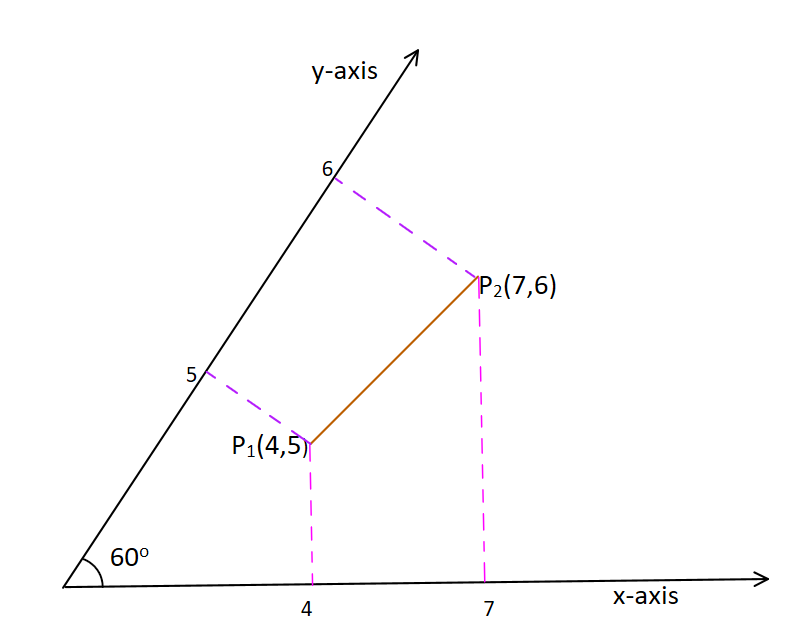
\includegraphics[height=5cm]{fig1.png}
  \end{frame}
  
}

%------------------------------------------------------------


\begin{document}

%The next statement creates the title page.
\frame{\titlepage}


%---------------------------------------------------------
%This block of code is for the table of contents after
%the title page
\begin{frame}
\frametitle{Table of Contents}
\tableofcontents
\end{frame}
%---------------------------------------------------------


\section{First section}

%---------------------------------------------------------
%Changing visivility of the text



%---------------------------------------------------------


%---------------------------------------------------------

\begin{frame}
\frametitle{Solution}
It can be solved by transforming the axes into rectangular coordinates as shown in figure \\
Let the transformed coordinates of \myvec{x_1\\y_1} \& \myvec{x_2\\y_2} be \myvec{x_3\\y_3} \& \myvec{x_4\\y_4} respectively.
\begin{figure}
    \centering
    \includegraphics[height=5cm]{fig2.png}
    \caption{Points defined on angular and rectangular axes}
    \label{fig:1}
\end{figure}
\end{frame}
%---------------------------------------------------------



%---------------------------------------------------------
%Highlighting text
\begin{frame}
From the figure,\\
x_3 = OX_1 + X_1X_3 = x_1+y_1\cos{60^{\circ}}\\
y_3 = OY_1\cos{30^{\circ}} = y_1\cos{30^{\circ}}\\
\begin{equation}
\myvec{x_3\\y_3} = \myvec{1 \ \cos{60^{\circ}} \\ 0 \  \cos{30^{\circ}}} \myvec{x_1\\y_1}\label{eq:1.0.2}   
\end{equation}
Similarly,\\
x_4 = OX_2 + X_2X_4 = x_2+y_2\cos{60^{\circ}} \\
y_4 = OY_2\cos{30^{\circ}}  =\ y_2\cos{30^{\circ}}\\
\begin{equation}
\myvec{x_4\\y_4} = \myvec{1 \ \cos{60^{\circ}} \\ 0 \  \cos{30^{\circ}}} \myvec{x_2\\y_2}\label{eq:1.0.3}
\end{equation}
The generalised equation for transformed coordinates $\myvec{x_t\\y_t}$ when the angle between axes '$\theta$' is,
\begin{equation}
\boxed{\myvec{x_t\\y_t} = \myvec{1   \ \  \cos{(\theta)} \\ 0 \ \ \sin{(\theta)}} \myvec{x\\y}}  \label{eq:1.0.123} 
\end{equation}
\end{frame}
%---------------------------------------------------------

\begin{frame}
Let the transformed point be $\vec{X_t}$, $\vec{T}$ be the transformation matrix and the point in angular axes be $\vec{X}$, \eqref{eq:1.0.123} can be written as
\begin{equation}
 \vec{X_t} = \vec{T} \ \vec{X}\label{eq:1.1.125}  
\end{equation}
Solving \eqref{eq:1.0.2} \& \eqref{eq:1.0.3} the transformed coordinates are,\\
\begin{align}
      \myvec{x_3\\y_3} = \myvec{\frac{13}{2}\\\frac{5\sqrt{3}}{2}};\ \myvec{x_4\\y_4} = \myvec{10\\3\sqrt{3}}\label{eq:1.0.8}    
 \end{align}
 The distance between points is a norm of the distance vector,
\begin{equation}
d = \norm{\vec{X_t_1}-\vec{X_t_2}} 
\end{equation}
\begin{equation}
d = \norm{\vec{T}(\vec{X_1}-\vec{X_2})}
\end{equation}
\begin{equation}
d = (\vec{X_1}-\vec{X_2})^\top \  \vec{T}^\top \  \vec{T} \ (\vec{X_1}-\vec{X_2}) = \sqrt{13} \label{eq:1.1.135}
\end{equation}
    
\end{frame}

%---------------------------------------------------------

\begin{frame}
\frametitle{Conclusion}

1. From the above solution, it can be concluded that the distance between points remains \alert{constant} irrespective of coordinate system.

2. It can also be concluded that the position vector of the points \alert{change} when the axes is transformed. 





\end{frame}
%---------------------------------------------------------


\end{document}
\begin{frame}
\frametitle{Solution}
Let the points be
\begin{equation}
\myvec{x_1\\y_1} = \ \myvec{4 \\5} \ ; \ \myvec{x_2\\y_2} \ = \myvec{7\\ 6} ; \theta = 60^{\circ} \label{1}
\end{equation}
The distance, d can be measured in angular axes (by cosine rule) by following equation,
 \begin{align}
 d = \sqrt{{\norm{\myvec{x_2\\y_2} - \myvec{x_1\\y_1}}}^2 +2\myvec{x_2-x_1\\0}^\top \myvec{y_2-y_1\\0}\cos{\theta}}\\ 
d = \sqrt{{\norm{\myvec{7\\6} - \myvec{4\\5}}}^2 +2\myvec{3&0} \myvec{1\\0}\cos{60^{\circ}}} 
\end{align}
\begin{align}
d = \sqrt{13} \ units \label{eq:1.0.4}   
 \end{align}
\end{frame}


%
Substituting \eqref{eq:1.1.5} 
\begin{equation}
d = \norm{\vec{T}(\vec{X_1}-\vec{X_2})} 
\end{equation}
\begin{equation}
d = (\vec{X_1}-\vec{X_2})^\top \  \vec{T}^\top \  \vec{T} \ (\vec{X_1}-\vec{X_2})  
\end{equation}
\begin{equation}
d = \sqrt{13} \ units  \label{eq:1.1.10}
 The distance between two points is norm of distance vector in rectangular coordinates\\
\begin{equation}
\norm{\myvec{x_3\\y_3} - \myvec{x_4\\y_4}} = \norm{\myvec{10\\3\sqrt{3}} -\myvec{\frac{13}{2} \\ \frac{5\sqrt{3}}{2}}} = \sqrt{13} \ units \label{eq:1.0.9}
 \end{equation}